\subsection{Syntax-number units connections}

\begin{figure*}[t]
    \centering
    \begin{subfigure}{0.49\textwidth}
            \centering
            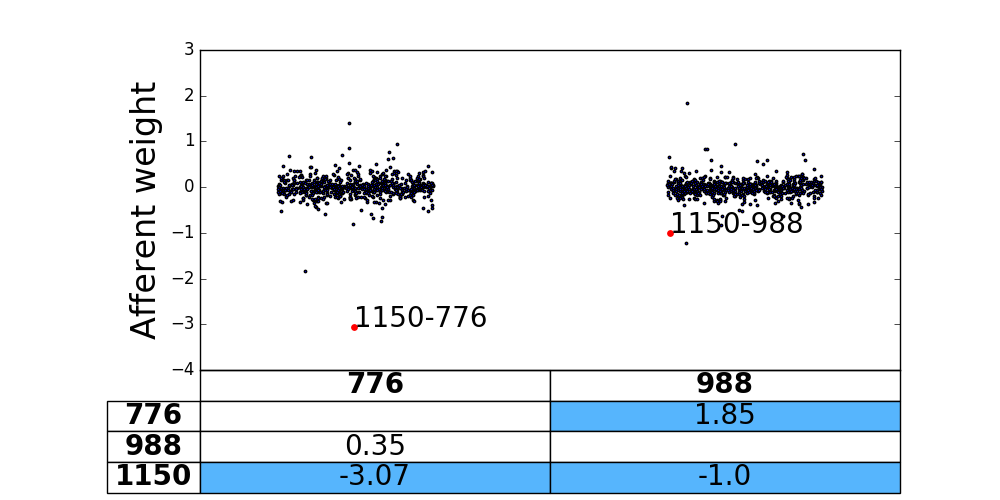
\includegraphics[width=\textwidth]{Figures/gate_Input_afferent_interactions.png}
            \caption{Input gate}
            \label{fig:interaction-input}
    \end{subfigure}
    \begin{subfigure}{0.49\textwidth}
           \centering
          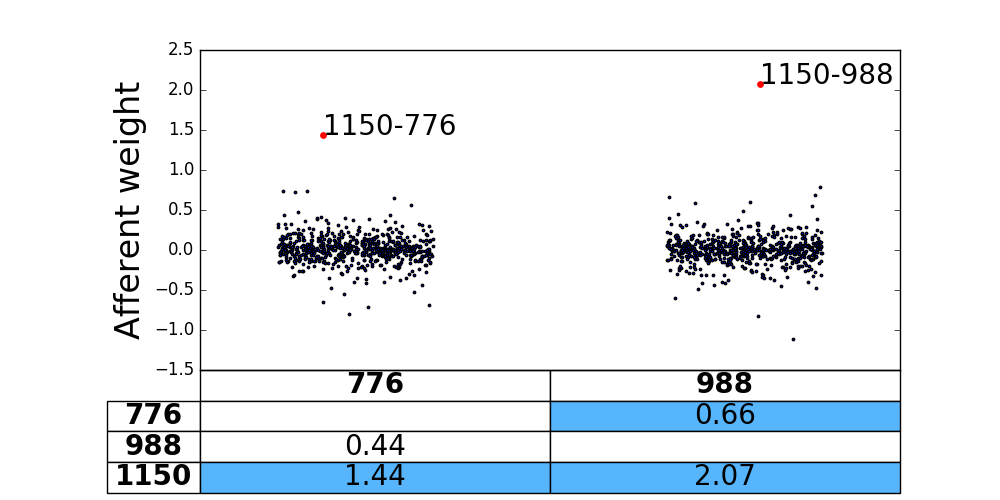
\includegraphics[width=\textwidth]{Figures/gate_Forget_afferent_interactions.png}
          \caption{Forget gate}
          \label{fig:interaction-forget}
    \end{subfigure}
\caption{Connectivity among the syntax unit \unit{2}{500} and LR-number units: \unit{2}{126}, \unit{2}{338}. Projecting units appear to the left of the table, and blue background represents that the corresponding value is an outlier ($|z-score|>3$). Weights from the syntax units are marked in red and are labeled on the distribution. }
\label{fig:interaction}
\end{figure*}

We finally look at the connections that were learned by the LSTM
between syntax unit \unit{2}{500}, which appears to be more closely involved in
tracking subject-verb agreement, and the number units, as well as at
the connections between the latter. For each unit pair, there are 4
connection types, one for each component of the target cell (to the 3
gates and to the memory cell). We focus on input and forget gates, as they control the flow and storage of number information.

Figures \ref{fig:interaction-input} and \ref{fig:interaction-forget} show the distributions of all afferent recurrent weights to the input and forget gates of the LR-number unit, scaled by the maximal activity $h_t$ of the pre-synaptic units during the nounPP task (for evaluating the effective input to the LR-units). We found that the weight values from the syntax unit to the forget gate of both \unit{2}{126} and \unit{2}{338} are exceptionally high compared to all other afferent connections in the network ($z-score=8,1, 11.2$, respectively), and exceptionally negative to their input gates ($z-score=-16.2, -7.2$). Since cell activity of syntax unit \unit{2}{500} is positive across the entire subject-verb dependency (e.g., Figure
\ref{fig:syntax-unit-double-subjrel}), the connectivity from the
syntax unit drives the number unit forget gates towards 1
($W^f_{776, 1150}h_{1150}>0$) and their input gates towards 0
($W^i_{776, 1150}h_{1150}<0$). Looking at the right-hand-side of
Eq.~(\ref{eq:update-rule}), this means that the first term becomes
  dominant and the second vanishes, suggesting that, across the entire
  dependency the syntax unit conveys a \textit{`remember flag'}
  to the number units, and, similarly, when the activity of the syntax
  unit becomes negative, it conveys an \textit{`update
    flag'} at the end of the dependency.

Last, we note that the reciprocal connectivity between the two LR-number units is always positive to both their input and forget gates (and significant from  \unit{2}{126} to \unit{2}{338}). Since their activity is negative throughout the subject-verb dependency (Figure \ref{fig:singular-unit} and \ref{fig:plural-unit}), this means that they are \textit{mutually inhibiting}, thus steering to an unequivocal signal about the grammatical number of the subject to the output layer.

